%% Default Latex document template
%%
%%  blake@rcs.ee.washington.edu

\documentclass[letterpaper]{article}

% Uncomment for bibliog.
%\bibliographystyle{unsrt}

\usepackage{graphicx}
\usepackage{lineno}
%\usepackage{fancyhdr}

%%%%%%%%%%%%%%%%%%%%%%%%%%%%%%%%%%%%%%%%5
%
%  Set Up Margins
\input{templates/pagedim.tex}

%
%        Font selection
%
%\renewcommand{\rmdefault}{ptm}             % Times
%\renewcommand{\rmdefault}{phv}             % Helvetica
%\renewcommand{\rmdefault}{pcr}             % Courier
%\renewcommand{\rmdefault}{pbk}             % Bookman
%\renewcommand{\rmdefault}{pag}             % Avant Garde
%\renewcommand{\rmdefault}{ppl}             % Palatino
%\renewcommand{\rmdefault}{pch}             % Charter


%%%%%%%%%%%%%%%%%%%%%%%%%%%%%%%%%%%%%%%%%%%%%%%%%
%
%         Page format Mods HERE
%
%Mod's to page size for this document
\addtolength\textwidth{0cm}
\addtolength\oddsidemargin{0cm}
\addtolength\headsep{0cm}
\addtolength\textheight{0cm}
%\linespread{0.894}   % 0.894 = 6 lines per inch, 1 = "single",  1.6 = "double"

% header options for fancyhdr

%\pagestyle{fancy}
%\lhead{LEFT HEADER}
%\chead{CENTER HEADER}
%\rhead{RIGHT HEADER}
%\lfoot{Hannaford, U. of Washington}
%\rfoot{\today}
%\cfoot{\thepage}



% Make table rows deeper
%\renewcommand\arraystretch{2.0}% Vertical Row size, 1.0 is for standard spacing)

\begin{document}
\setpagewiselinenumbers        %  Line numbers for edits to drafts.
\modulolinenumbers[1]          %  number every N lines

% \linenumbers                   %  start numbering lines here

\title{--- Advanced Oscilloscope ---}

\author{ECE 474 \\
        Blake Hannaford\\
        Department of Electrical Engineering \\
        The University of Washington
}

\date{\today}

\maketitle

\section{The 10x Probe: Theory}
The 10x oscilloscope probe (or probe setting if switchable) actually {\it divides} the signal by 10.
Why would we want to do that (especially for weak signals)??

The answer is that sometimes we have strong enough
signals but the `scope has limited {\it bandwidth}.
The 10x probe was invented to trade off some signal gain ($10x=-20dB$ specifically) for higher
frequency response.   ``10-x'' refers to the fact that the scope changes its vertical {\tt Volts-per-Division}
setting so that we don't have to do the mental math when using a 10x probe.

How does this work?   First we have to understand what the input circuit of an oscilloscope looks:

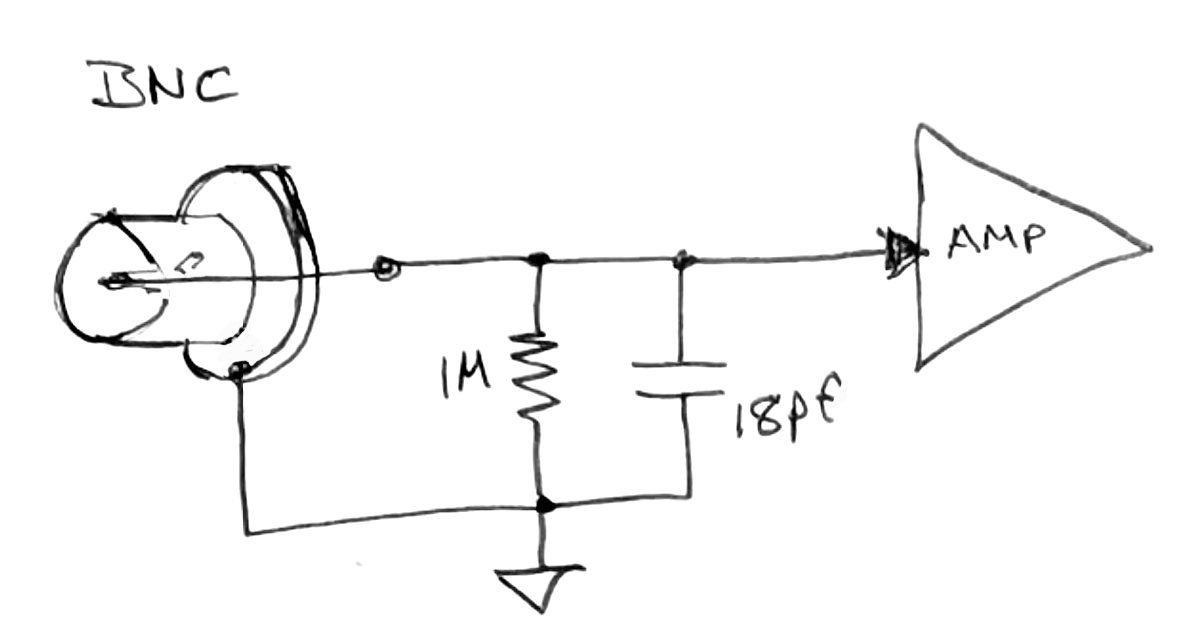
\includegraphics[width=75mm]{ID24734.png}

Here we show the amplifier input as idealized (drawing no current from the signal) but a $1M\Omega$
resistor in parallel with an $18pF$ capacitor.   These represent the non-ideal
electrical properties of the input
and in fact are calibrated/standardized and the values are usually printed on the front of the scope.

Note that depending on other impedances like the source impedance of the signal and the cables,
this could create a pole at

\[
\frac{1}{RC} = 55.6 k rad/sec = 349kHz
\]

quite limiting for today's fast logic.

Here's a diagram of a signal hooked up to this input via a basic wire (e.g. a 1X probe).

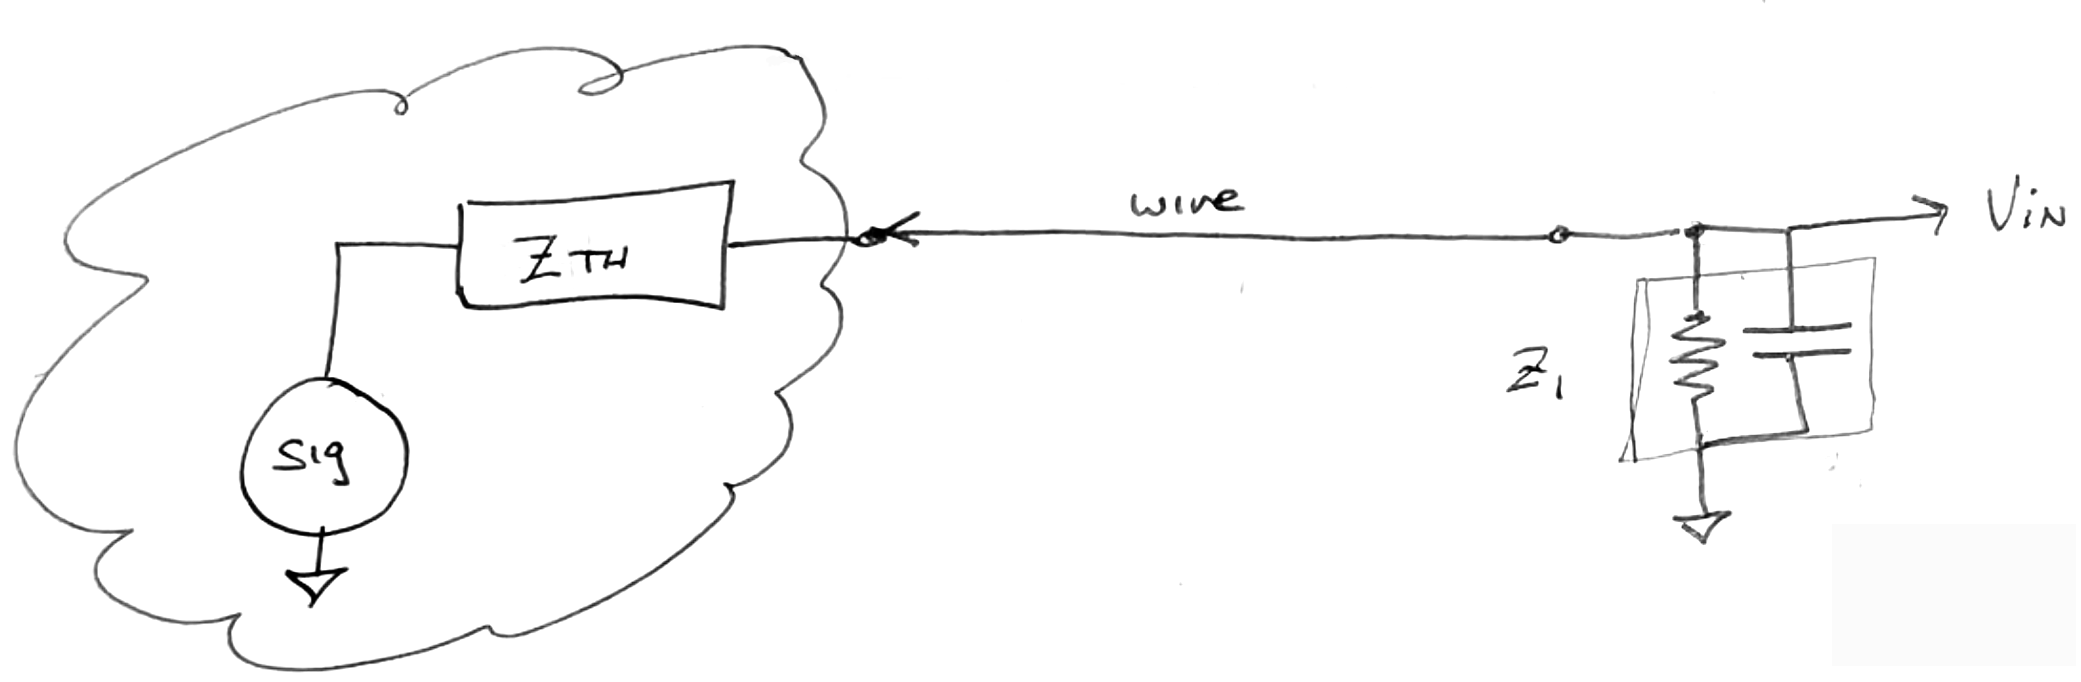
\includegraphics[width=120mm]{VK11711.png}

$Z_{Th}$ accounts for properties of the probe cable, including defects.

Suppose your probe touches a test point in a PCB.
$Z_{Th}$ comes from any number of random (but usually small) inductances and capacitances distributed
in the PCB wiring.
It is really hard for us to know these values and model them.
But they {\it will}
affect the measurement.


The load seen by the signal is  $Z_{Th} + R||C$.
This load draws current, and the oscilloscope's measured voltage, $V_{in}$,
will be dropped by
the Thevenin impedance of the signal source, $Z_{Th}$.


In fact, considering this is a voltage divider,
the voltage going into the
scope amplifier will be
\[
V_{in} = V_{signal}\frac{Z_1}{Z_{Th}+Z_1}
\]
but $Z_{Th}$ is basically unknown and very hard to control.


Working out the impedance, $Z_1$:
\[
Z_1 = R||\frac{1}{Cs} = \frac{R/Cs}{R+\frac{1}{Cs}} = \frac{1}{(s+\frac{1}{RC})}
\]

Consider adding a series impedance inside the probe, $Z_2$:

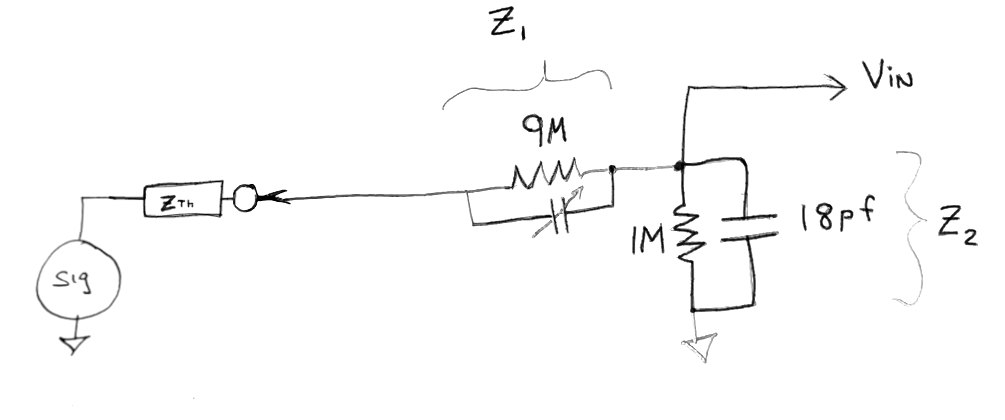
\includegraphics[width=90mm]{SD5923.png}

or more abstractly:

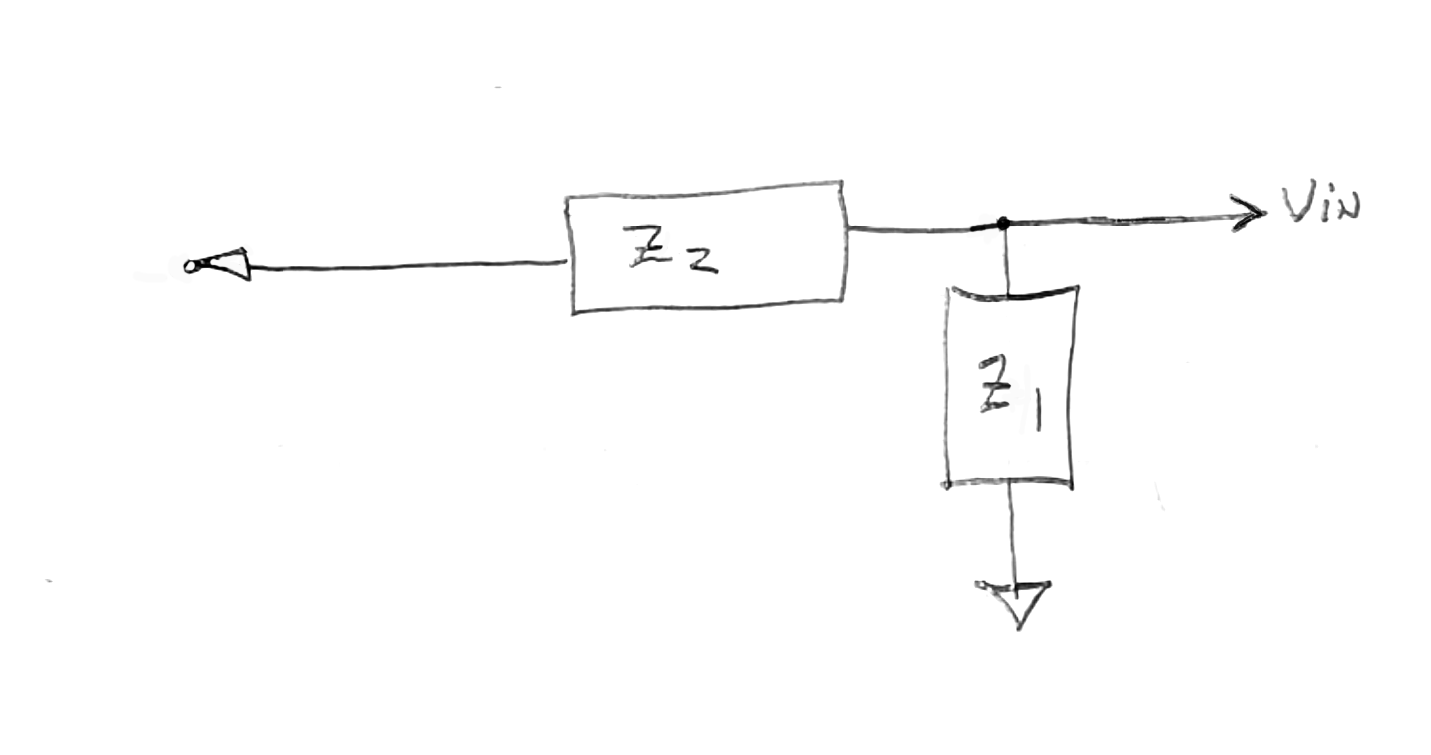
\includegraphics[width=90mm]{FS23983.png}


Now our voltage divider is
\[
V_{in} = V_{signal}\frac{Z_1}{Z_{Th}+Z_2+Z_1}
\]

and suppose we make $Z_2=9Z_1$, nine times bigger than $Z_1$.

Now we have
\[
V_{in} = V_{signal}\frac{Z_1}{Z_{Th}+10Z_1}
\]

We've made the input impedance of the scope 10x higher so we drop ~10x less from the parasitic and unknown
$Z_{Th}$.

Now we can look at the voltage divider assuming $Z_{Th} = 0$ where
 we {\bf assume} that the new impedance totalling
$Z_1+9Z_1=10Z_1$ is $>> Z_{Th}$.

\[
V_{in} = \frac{Z_1}{9Z_1+Z_1} = \frac {1}   {10}
\]

The result has a flat frequency response!  We've reduced the frequency dependent effects of the
mysterious $Z_{Th}$ by 10x.

\section*{Calibrating your 10x probe.}

The above analysis is great, but it   is sensitive to component tolerances, especially for the capacitor in
$Z_2$ (the 10x probe).   If you look at the base of your probe, you can see a little hole.
In this hole is the screw head for an adjustable capacitor.
The probe kit comes with a special small blade screwdriver.

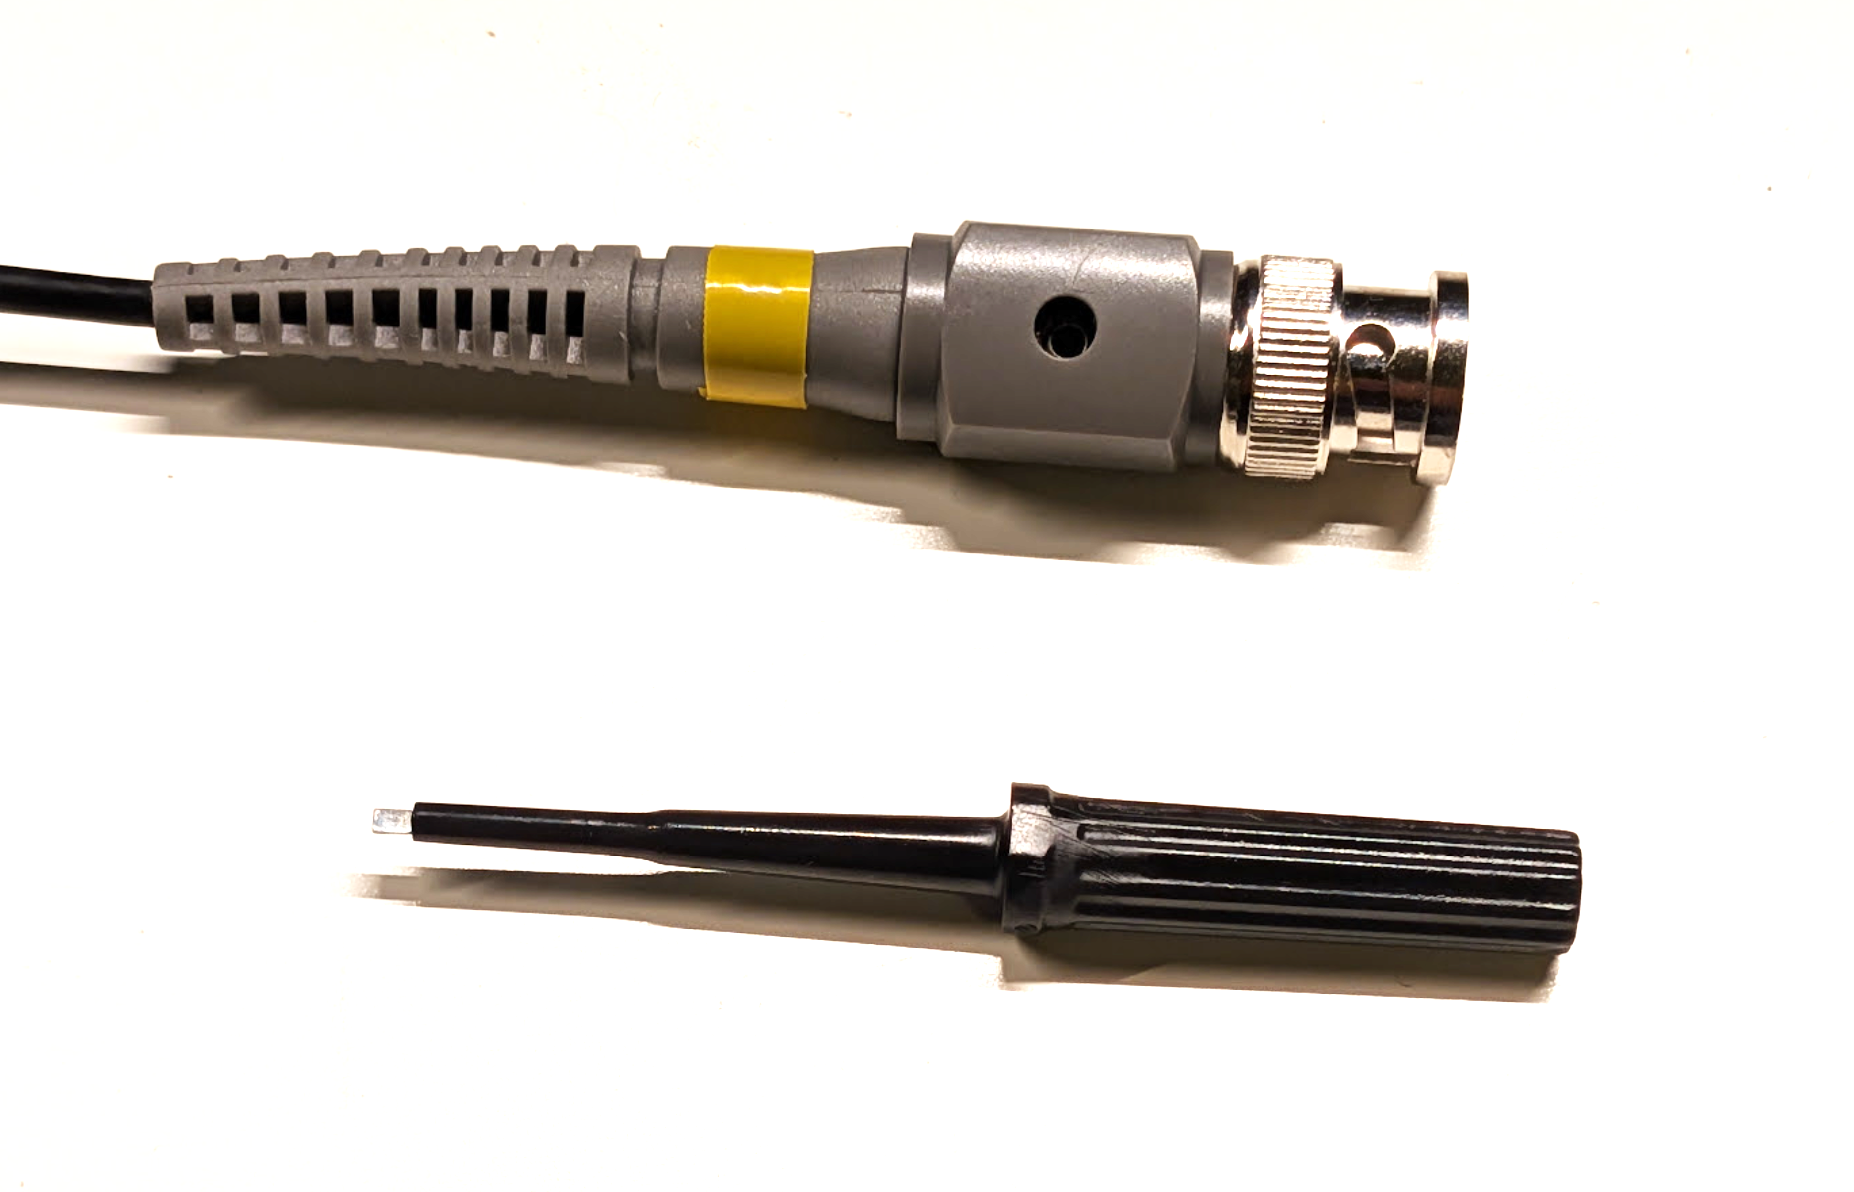
\includegraphics[width=90mm]{MN38817.png}


The screwdriver is mostly plastic, but
has a tiny metal blade.  This minimizes the change in capacitance when the blade contacts the screw.

To calibrate your 10x probe, set up the scope and connect it to a logic signal square wave.   Ground the ground clip as well.   Many oscilloscopes have a little terminal which outputs a square wave for this
purpose.

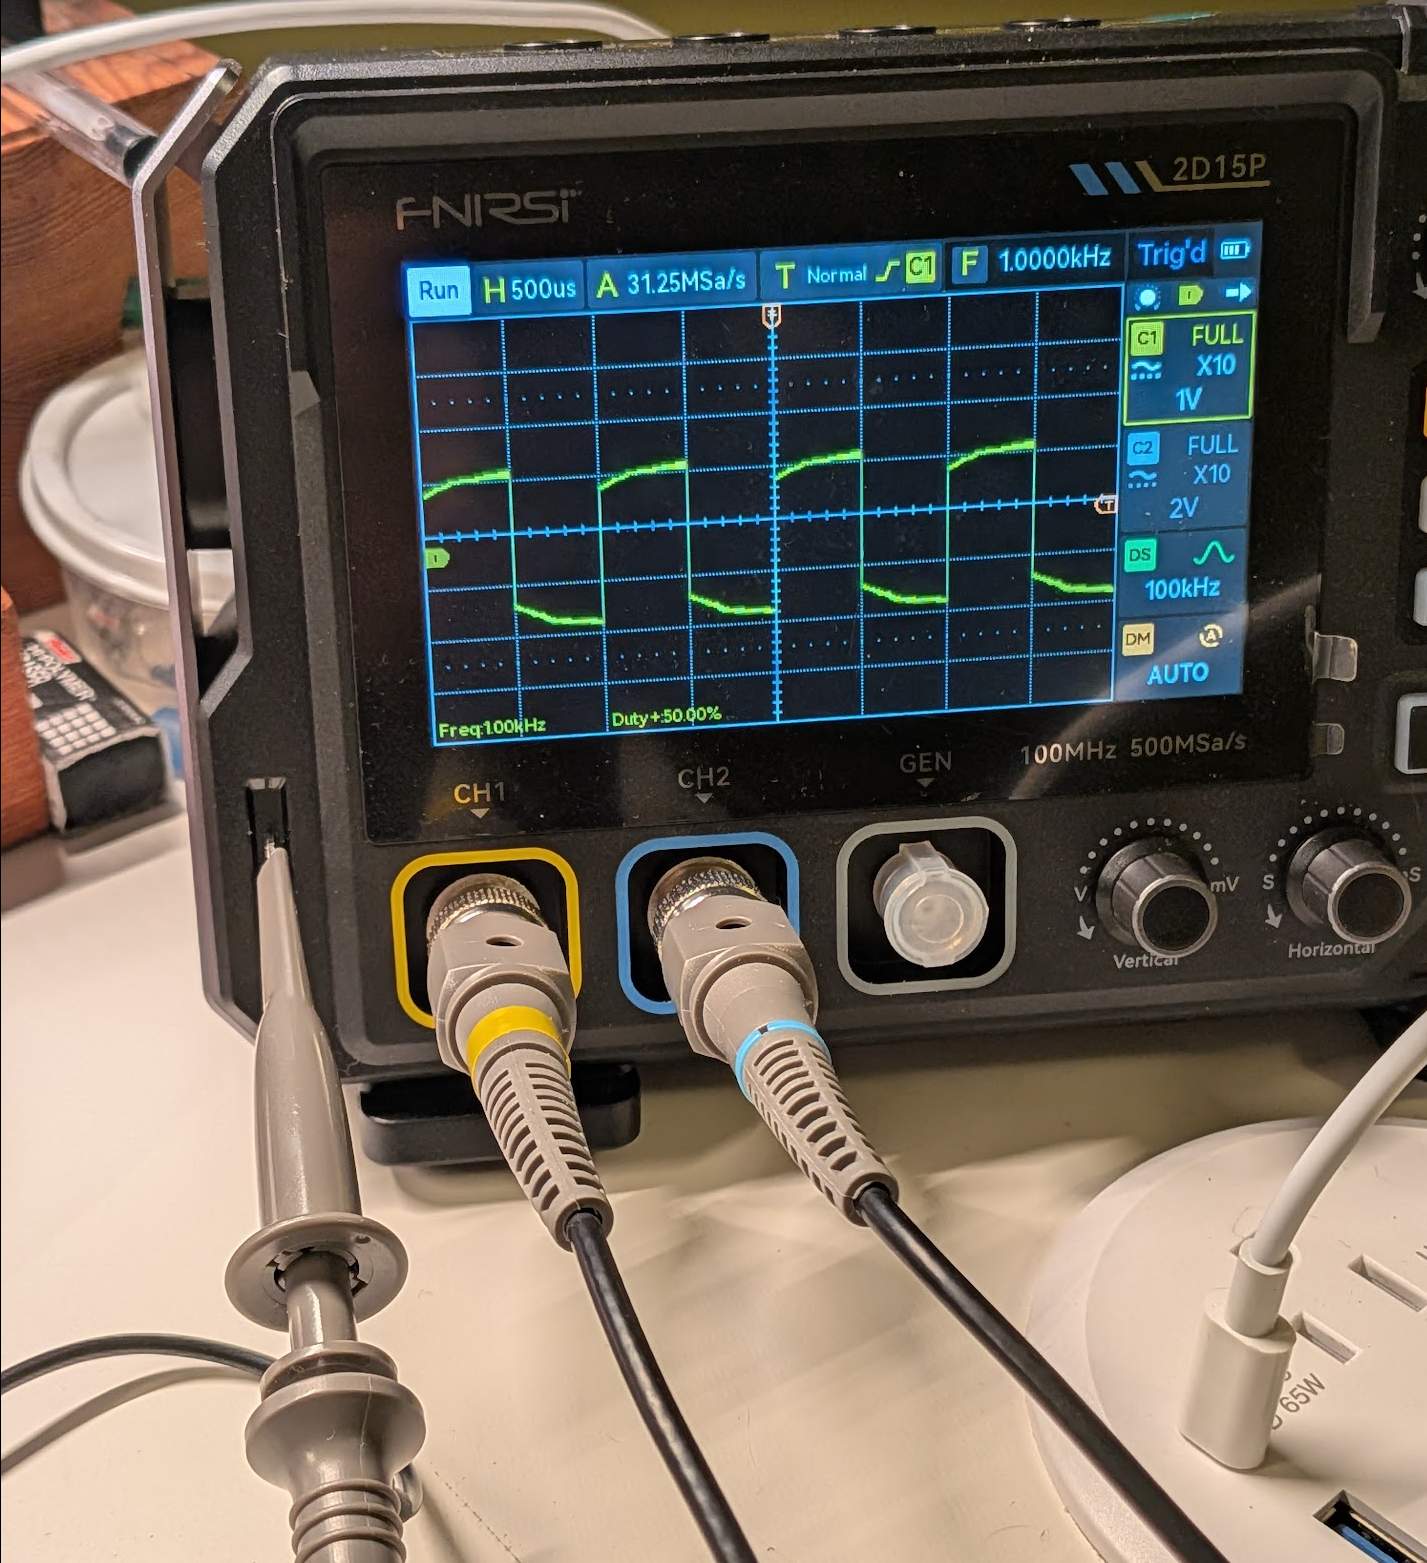
\includegraphics[width=90mm]{JG31951.png}

The probe is hooked up to the scope's calibration output clip (lower left of scope) and
the wave is distorted because the 10x probe is out of adjustment

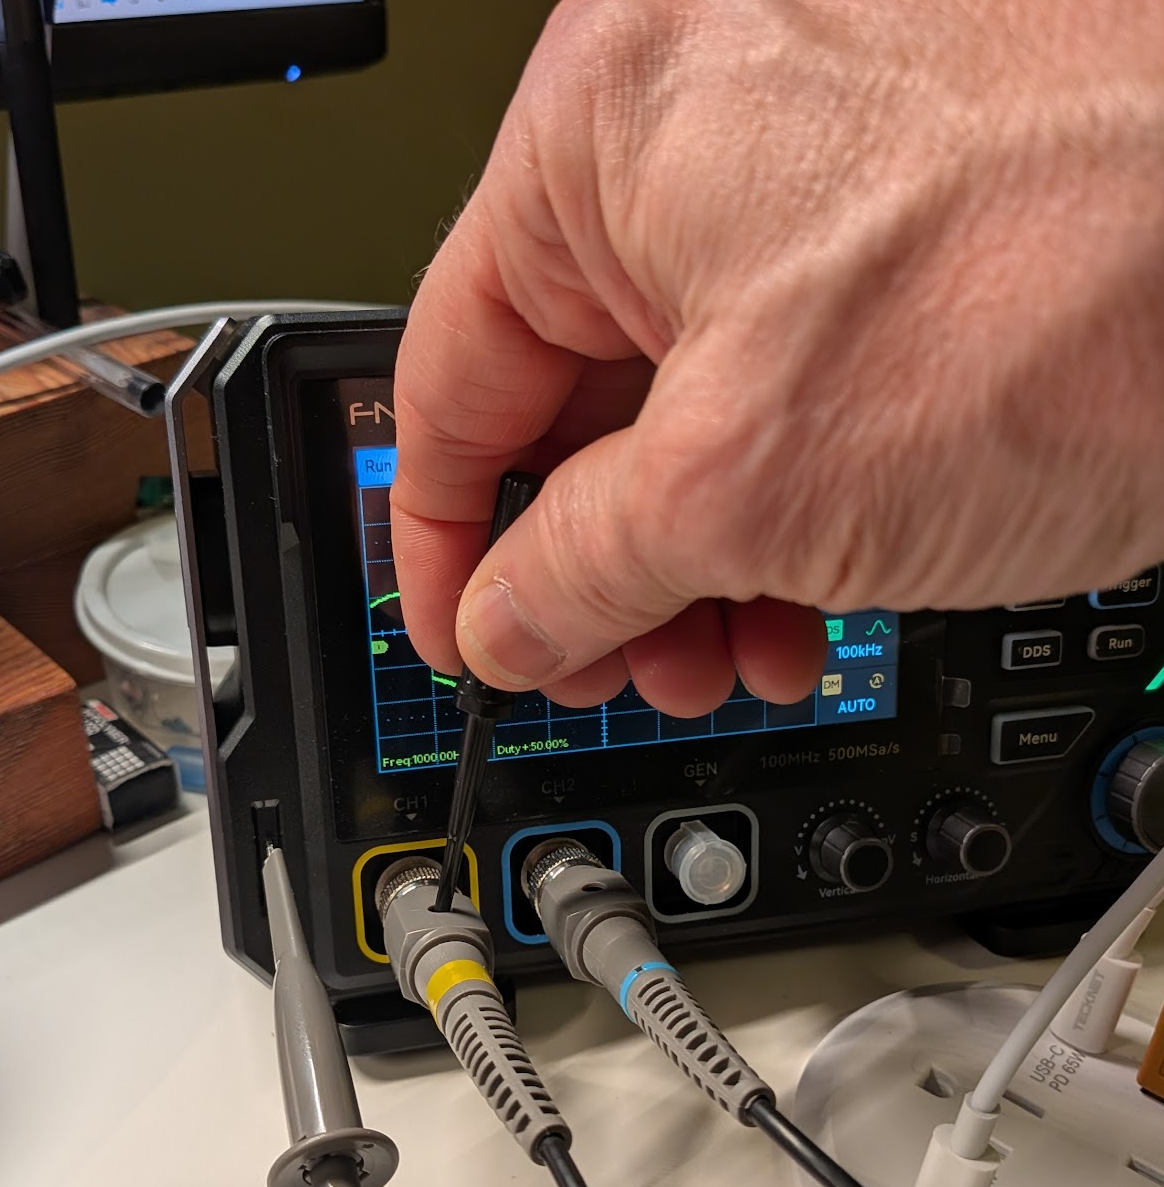
\includegraphics[width=90mm]{RE14019.png}

Gently turn the screw back and forth by small amounts to square-up the wave (we assume the calibration wave
output is perfect.)  It takes just seconds.

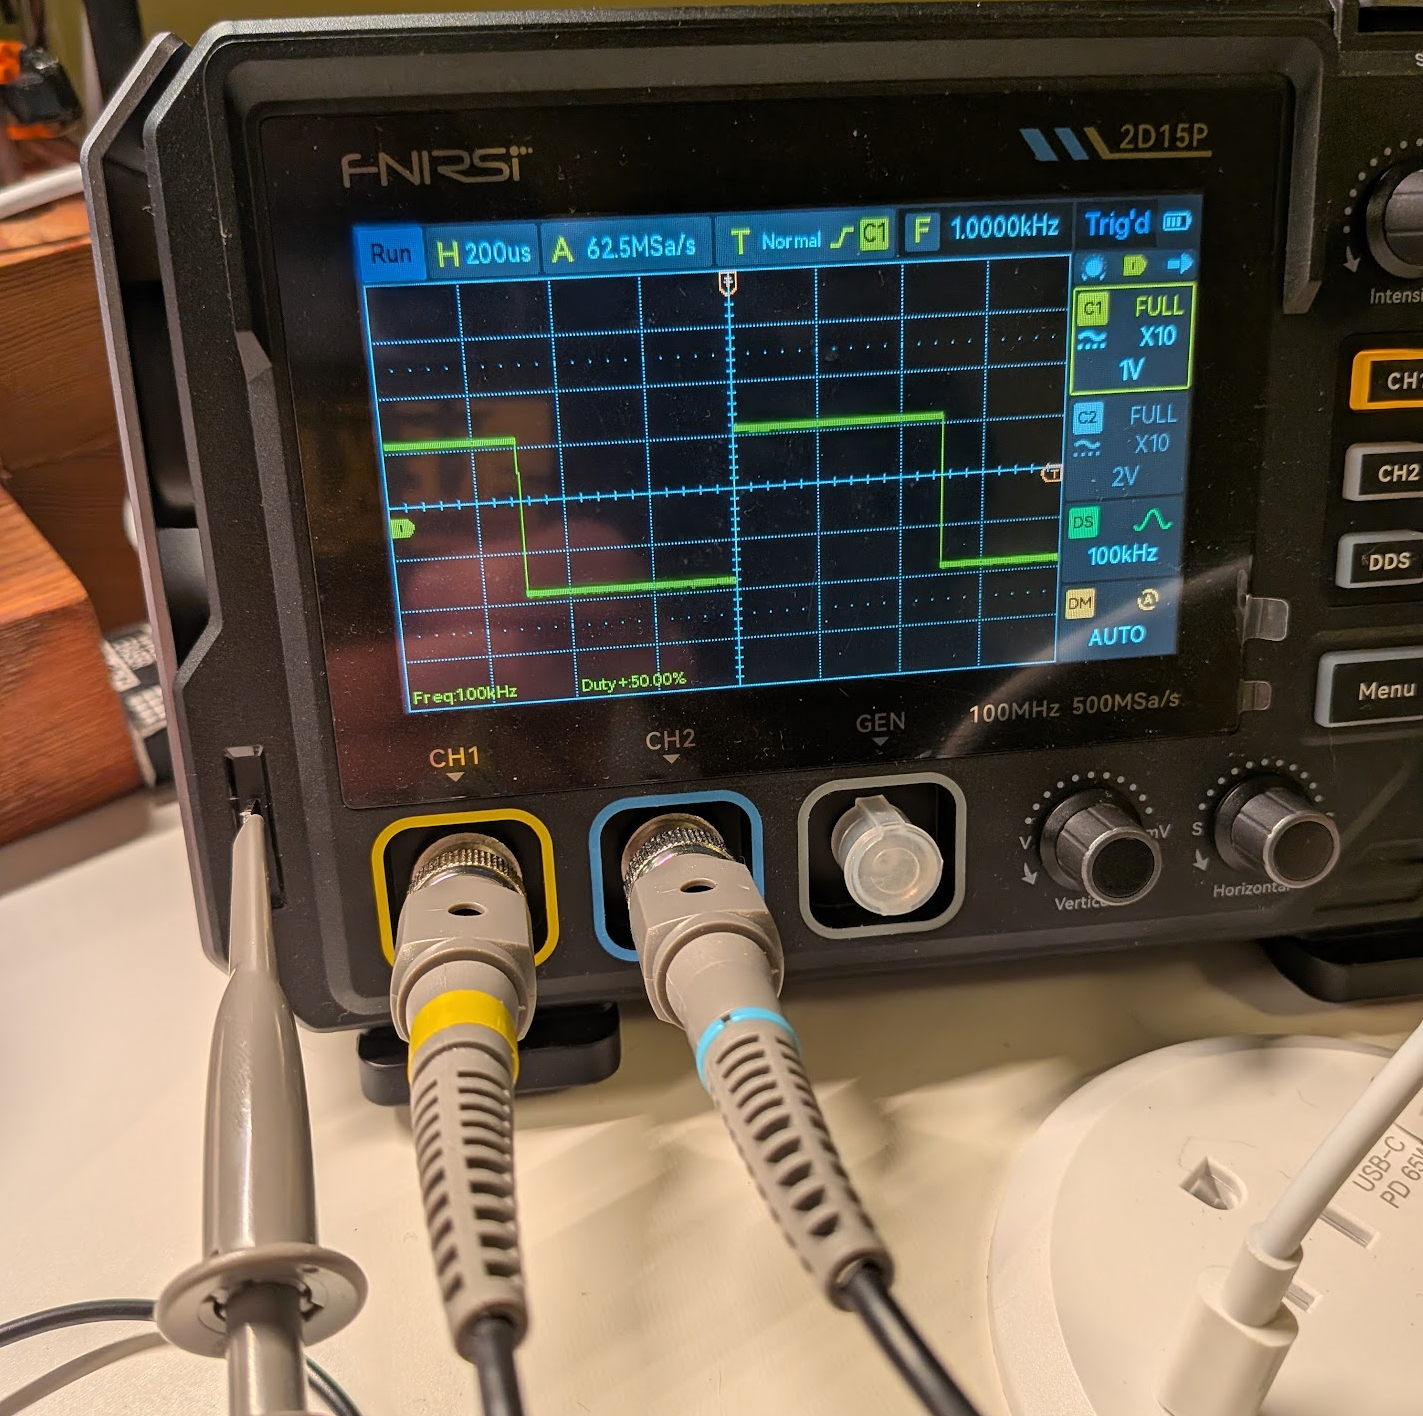
\includegraphics[width=90mm]{BE67977.png}

Now the wave is a perfect rectangle ... {\bf satisfying}.
\vspace{0.15in}

As seen here, if your probe is out of adjustment, the square wave will be distorted (as though it has been
put through a high-pass or low-pass filter - which it has!).  This is
because the probe's capacitor is not yet exactly right to cancel the capacitance inside the scope.  A little
tweak to the adjustment screw with the special screwdriver will trim up the pulses to perfect little
rectangles (which means you get the most accuracy and frequency response for any signal).
You might need to readjust your probe if you move it to a different scope.




%  Use name of bibliography files without .bib extension
%\bibliography{brl}
\end{document}

